\documentclass[a4paper, 10pt]{article}
% General document formatting

% Related to math
\usepackage{amsmath,amssymb,amsfonts,amsthm}

\usepackage{fullpage} % Package to use full page
\usepackage{parskip} % Package to tweak paragraph skipping

\usepackage[utf8]{inputenc}

\usepackage{enumitem,color,times,hyperref,graphicx,fourier-orns}
\usepackage[capitalise,noabbrev]{cleveref}

%------
%% define reviewer box
\newcounter{reviewer}[section]
\newenvironment{reviewer}{
    %% reviewer
    \refstepcounter{reviewer}\par\medskip
    \noindent \textbf{\underline{\textsc{Reviewer}~\thereviewer}:}
    %% define comment box
    \newcommand{\comment}[1]{\item{##1}}
    %% define response box
    \newcommand{\resp}[1]{\par\textit{##1}}
\begin{enumerate}[leftmargin=*]}
{\end{enumerate}}
%------

%% define submission no/title here
\newcommand{\subnum}{A001}
\newcommand{\subtitle}{my paper}
\newcommand{\opening}{
Dear Editor,

Thank you for the opportunity to revise and resubmit our paper ``\textsc{\subtitle}'' (\subnum).

}

%% horizontal seperatro
\newcommand{\mysep}{
    \begin{center}
        \huge
        $\ast$\hspace{1em}$\ast$\hspace{1em}$\ast$
    \end{center}
}



%%%%%%%%%%%%%%%%%%%
\title{\vspace{-5ex}\textsc{Response to Reviews for ``\subtitle'' }}
\author{A, B, C}
\date{\today}

\begin{document}
\maketitle

\opening

\mysep


\begin{reviewer}
    \comment{i think that ...}
    \resp{
	yes i know.
	\begin{figure}[!hb]
	\centering
	    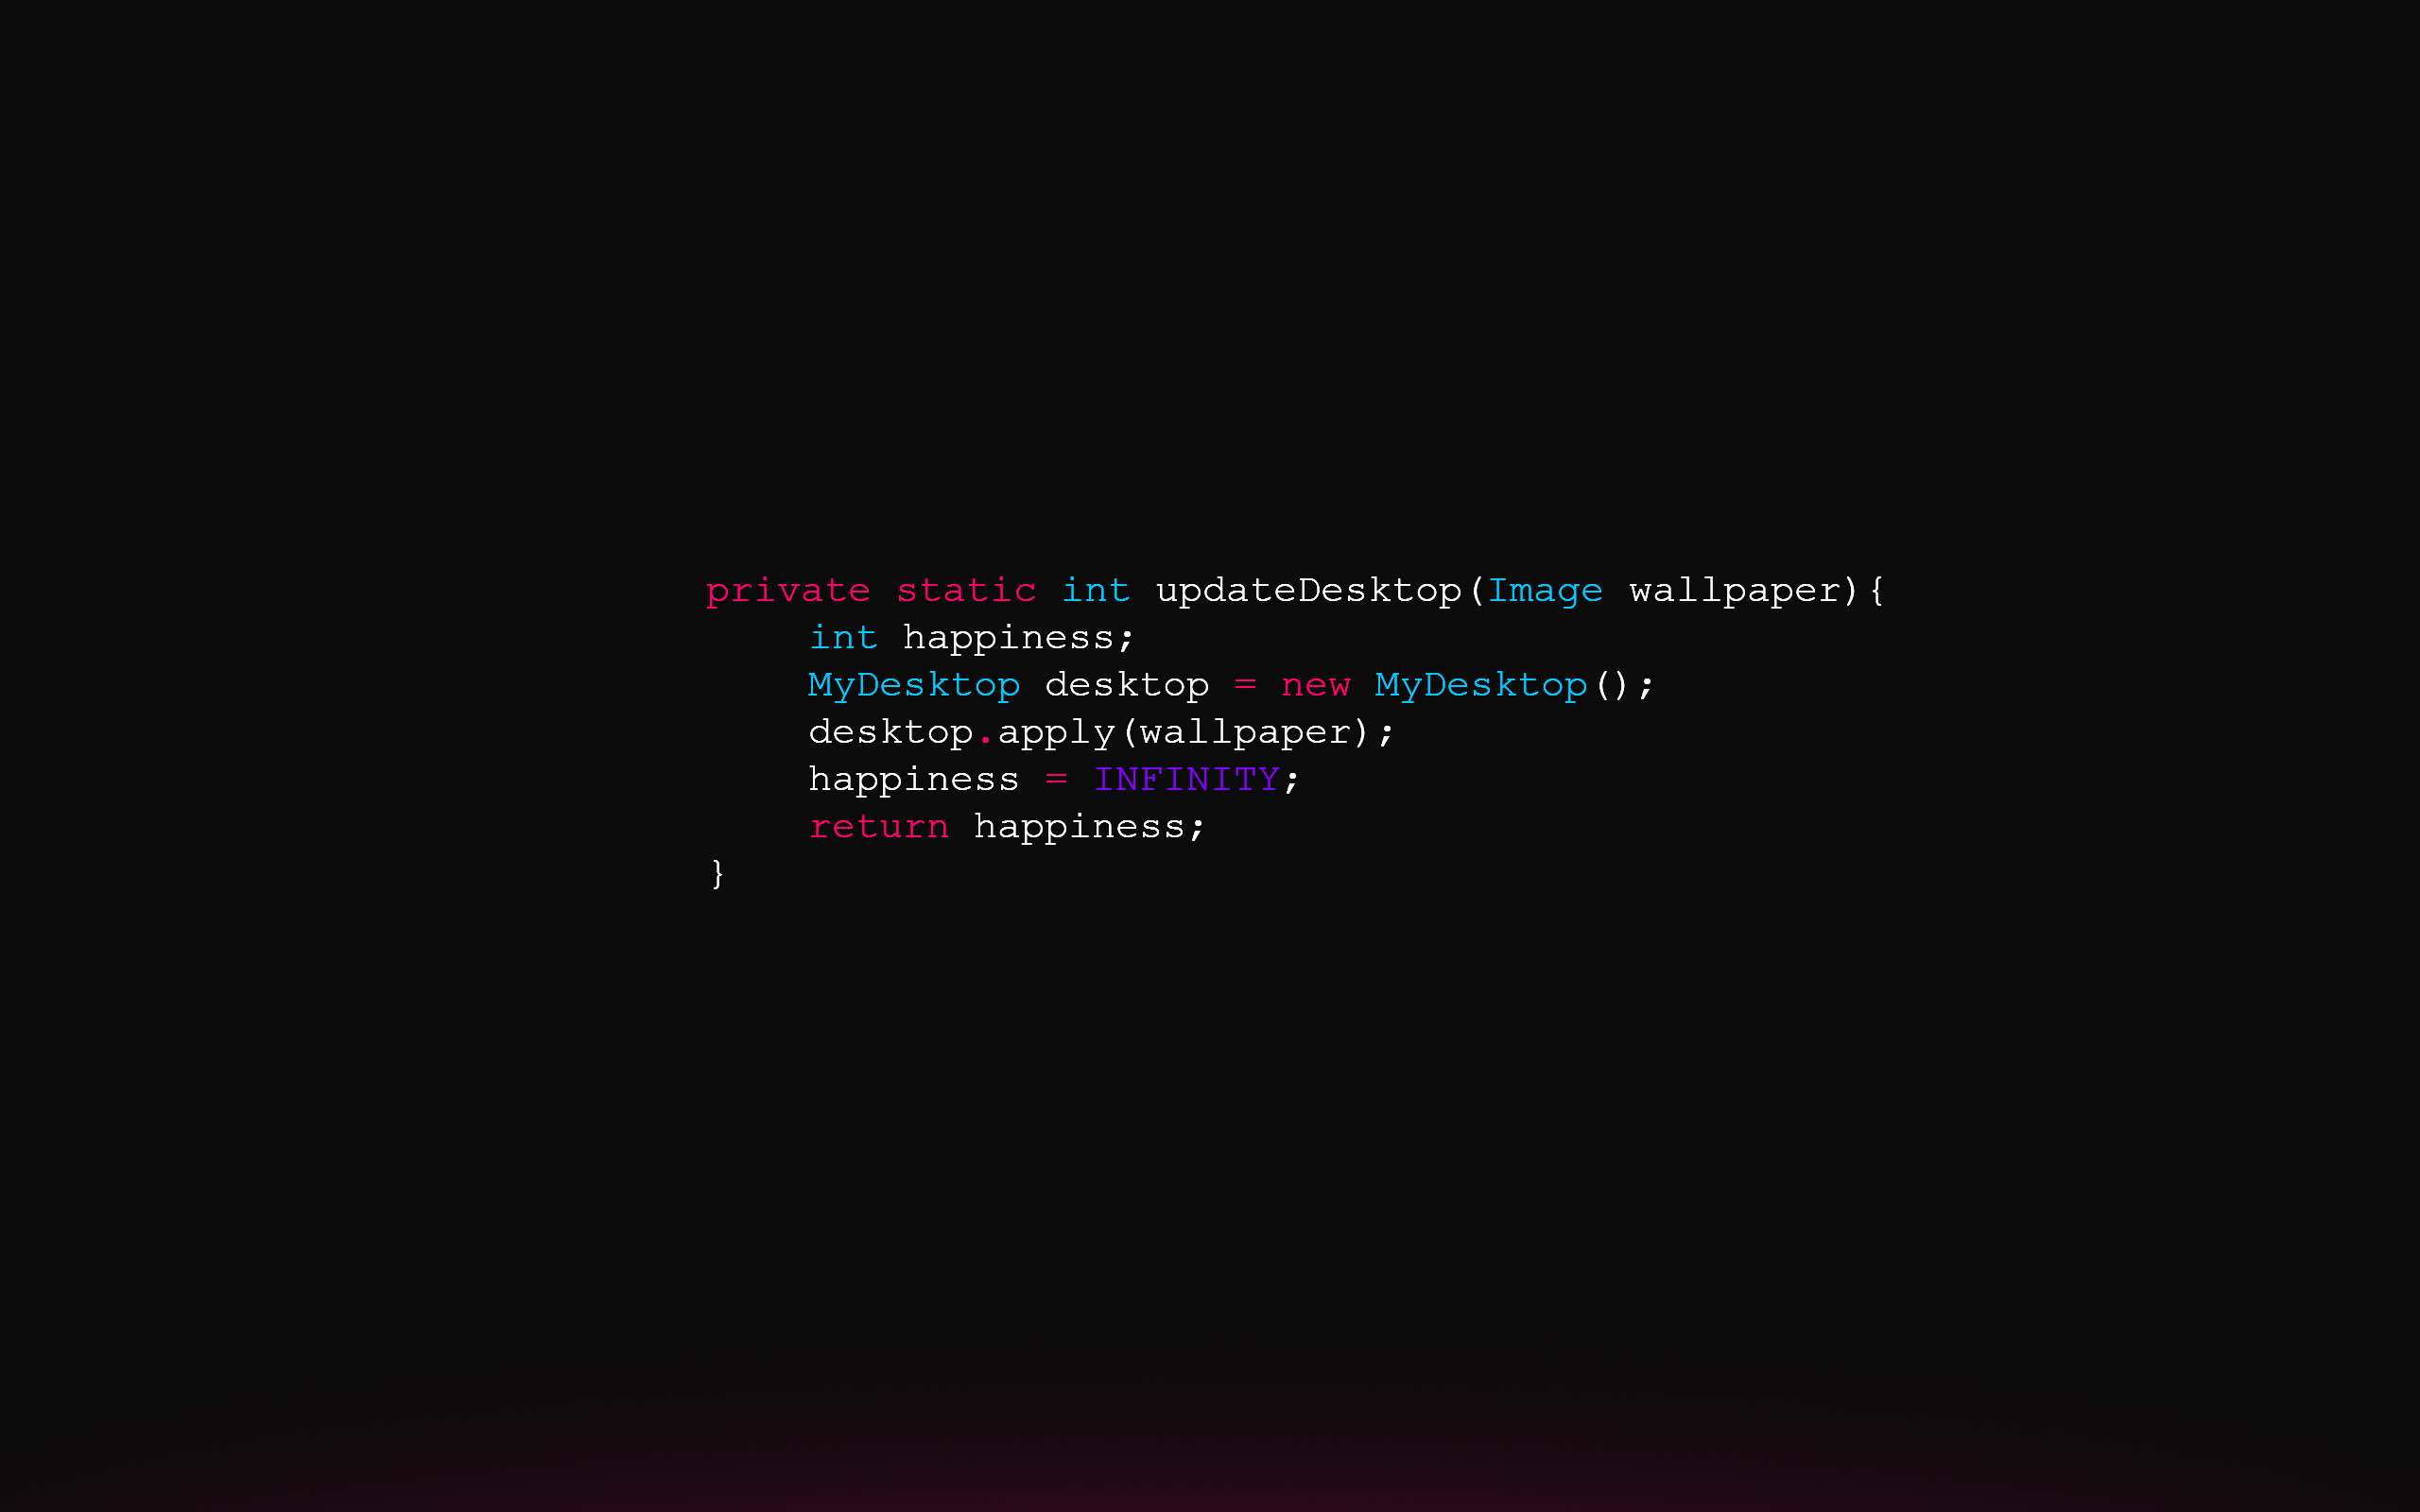
\includegraphics[width=0.5\columnwidth]{test}
	\end{figure}
    }
    %%
    \comment{i think that ...}
    \resp{
	thank you.
	\begin{figure}[!hb]
	\centering
	    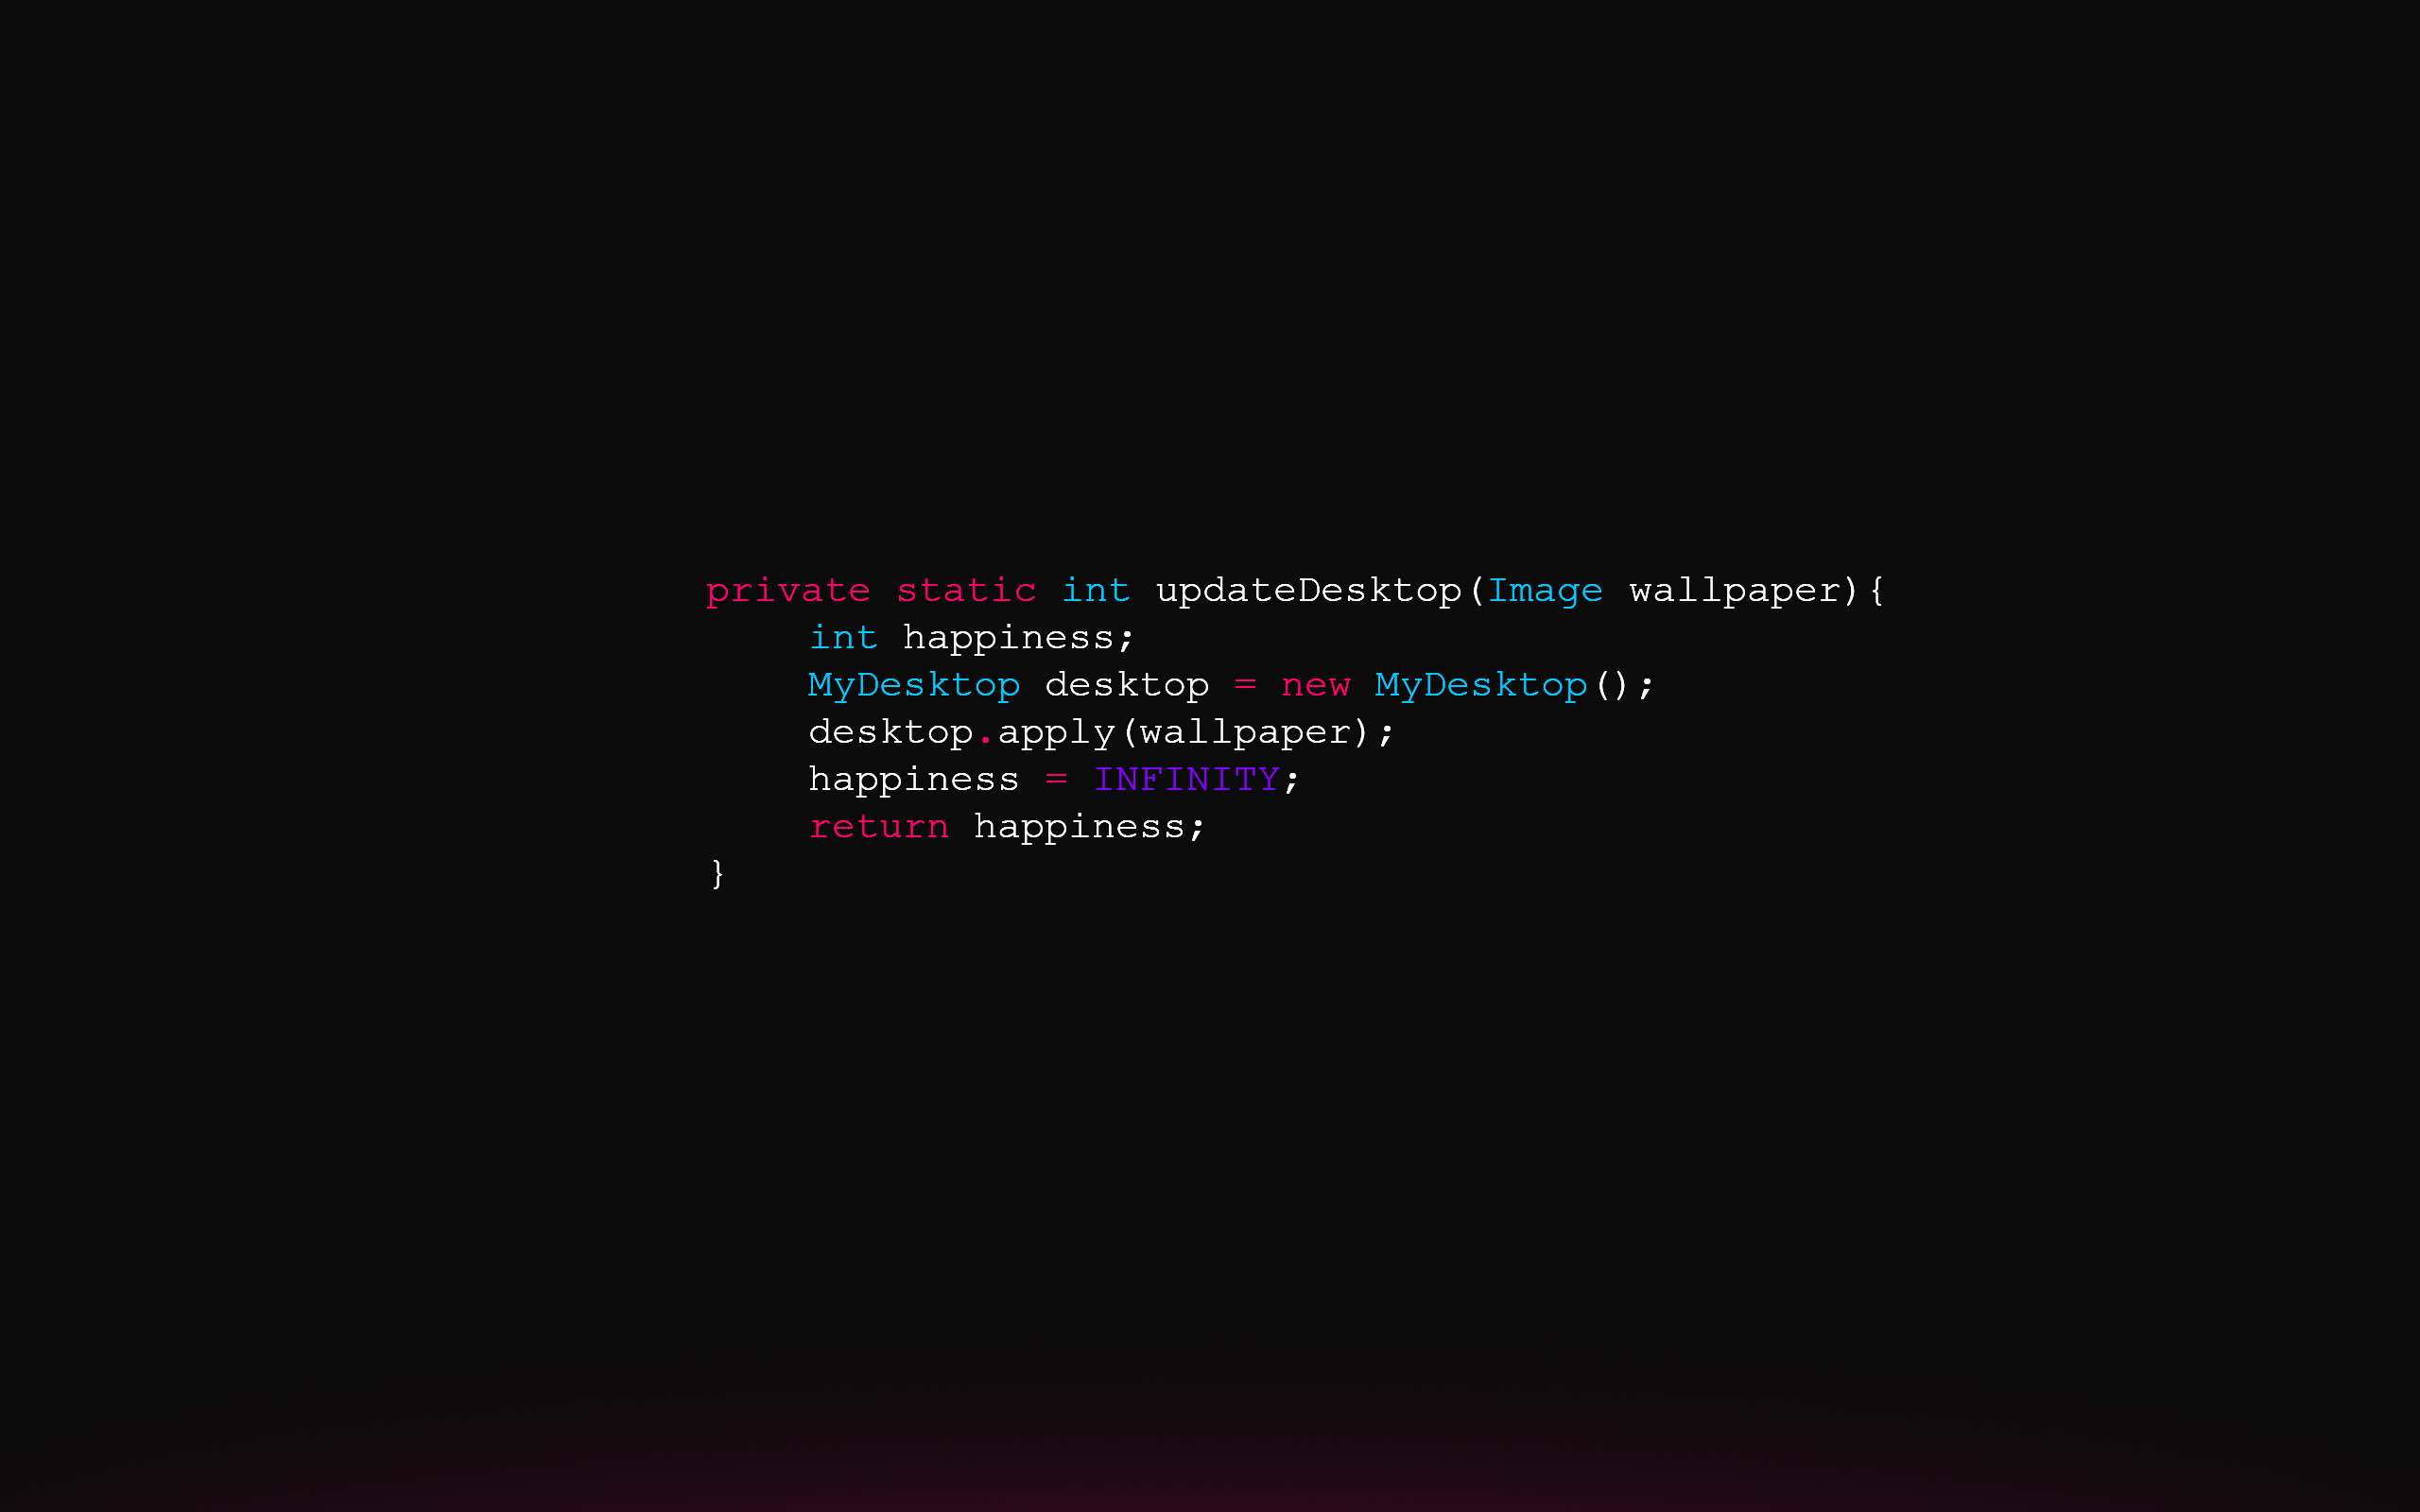
\includegraphics[width=0.5\columnwidth]{test}
	\end{figure}
    }
\end{reviewer}

\begin{reviewer}
    \comment{i think that ...}
    \resp{
	yes i know.
	\begin{figure}[!ht]
	\centering
	    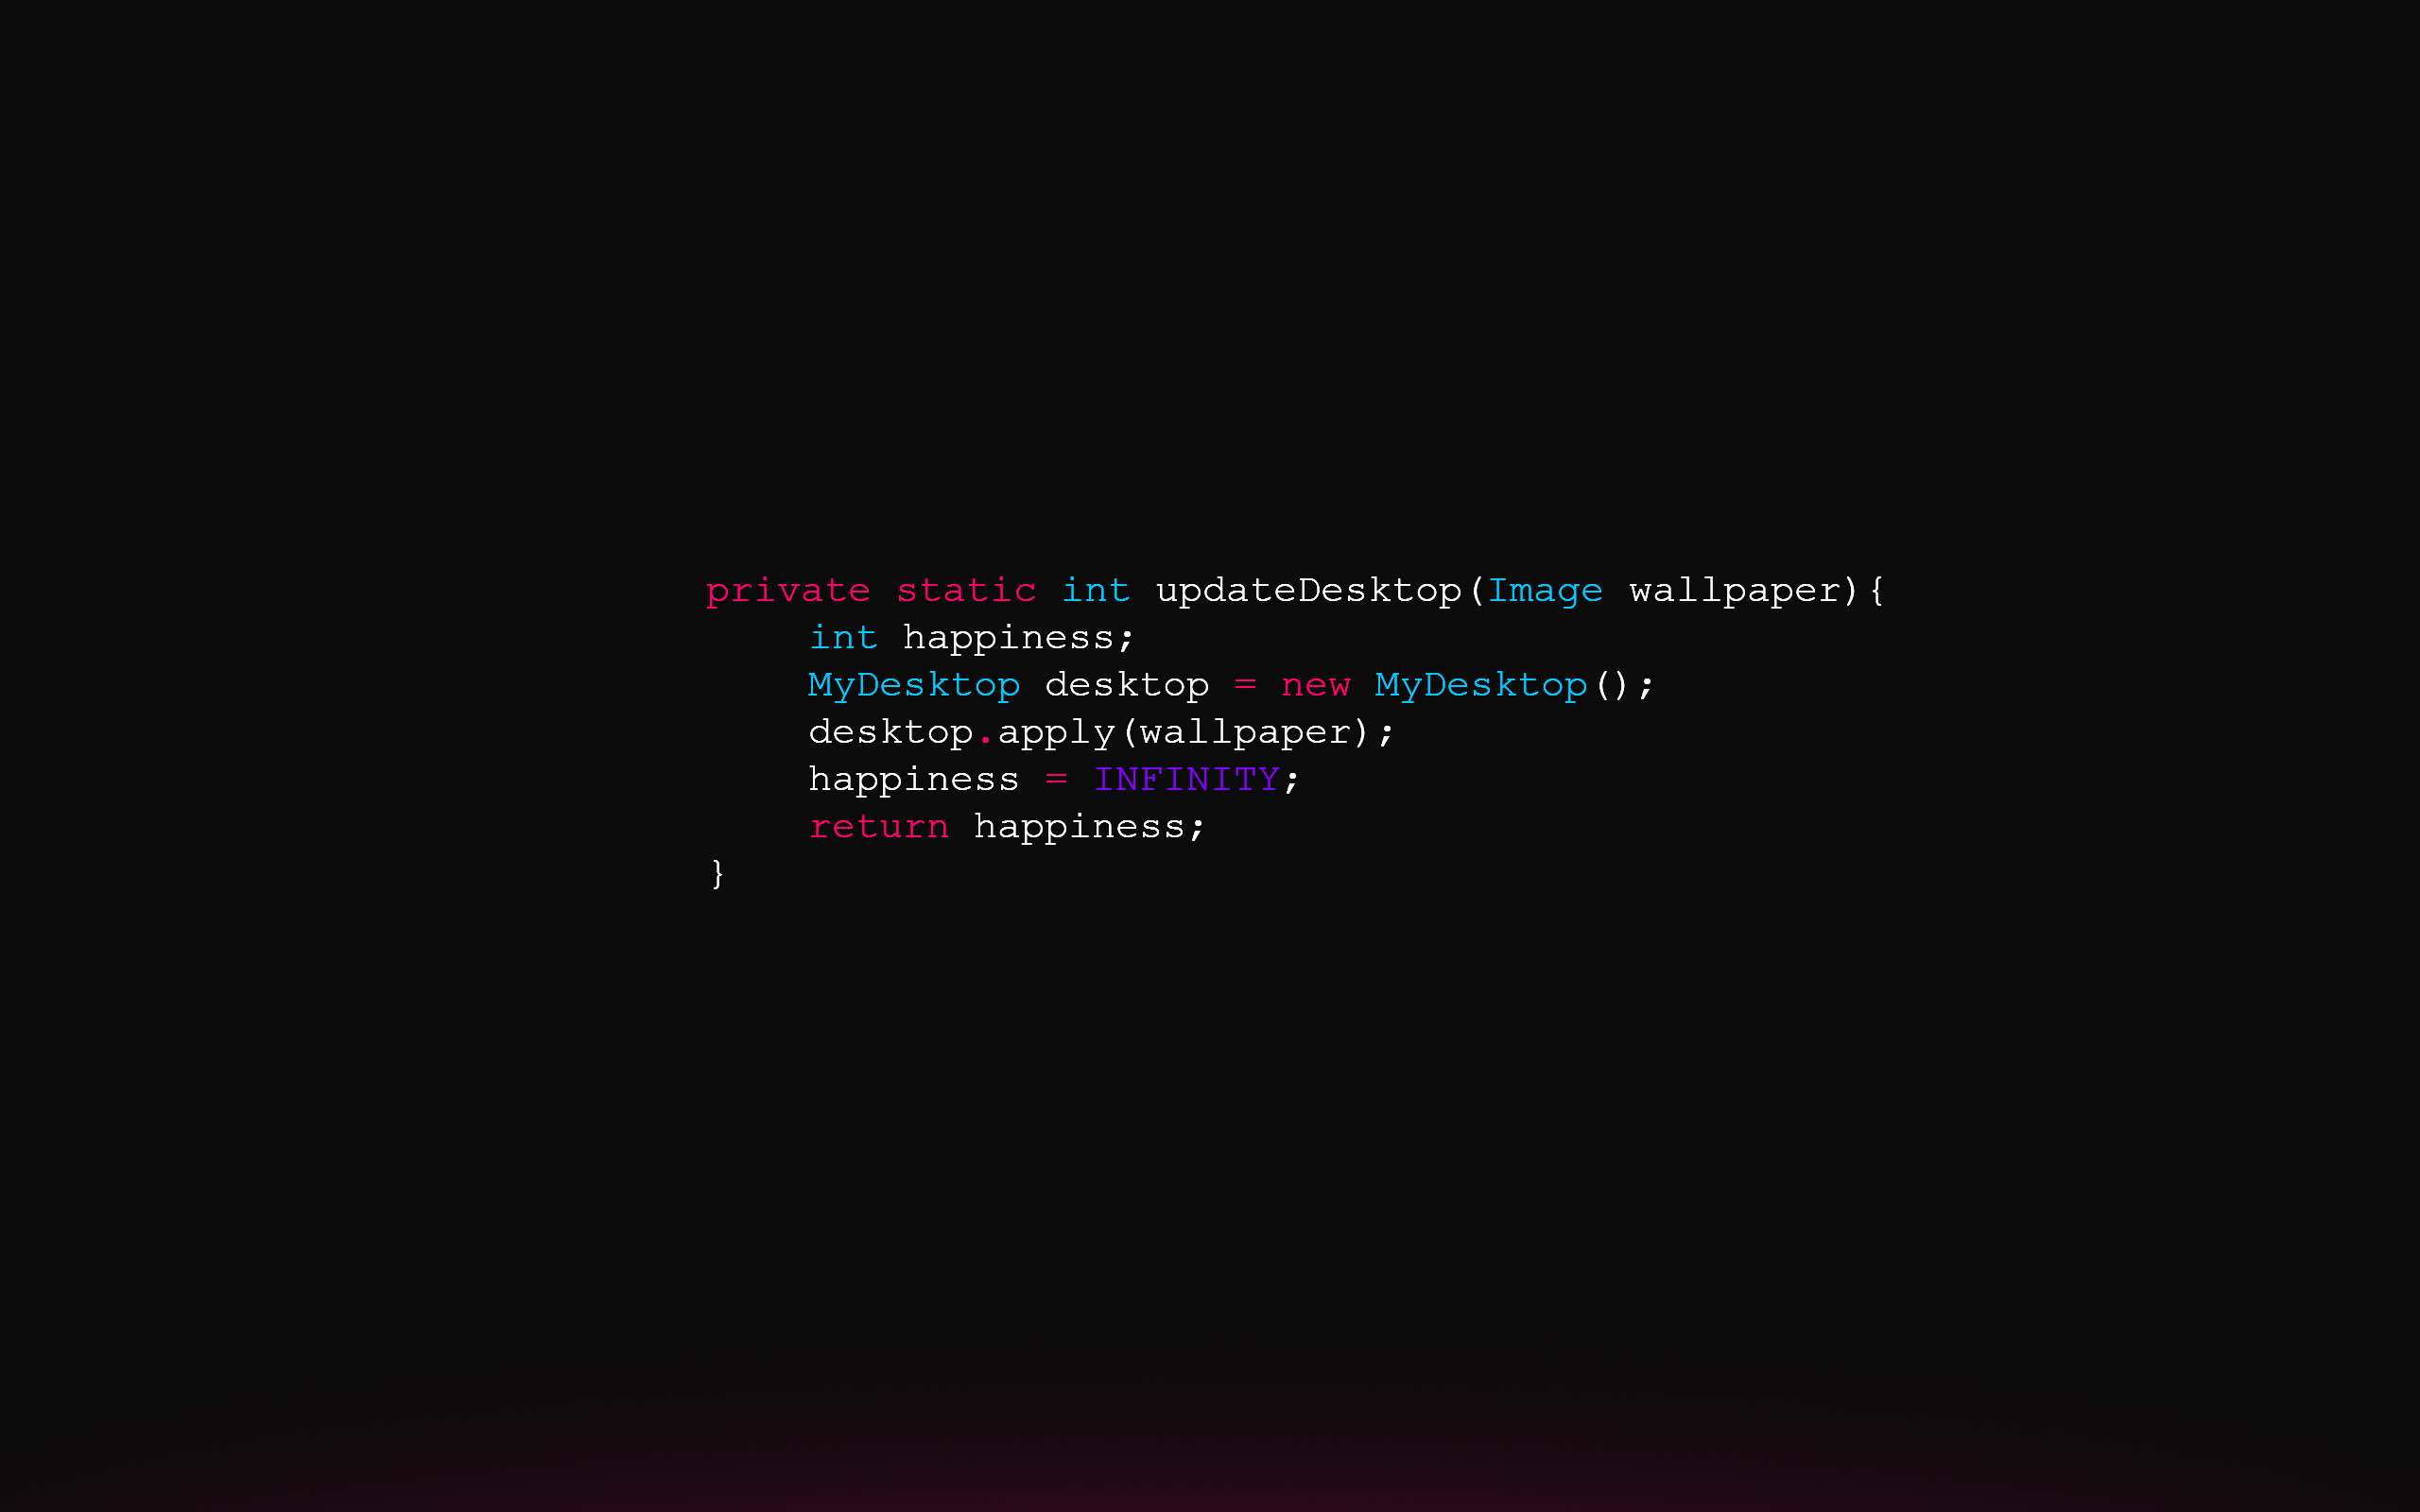
\includegraphics[width=0.5\columnwidth]{test}
	\end{figure}
    }
    %%
    \comment{i think that ...}
    \resp{
	thank you.
    }
\end{reviewer}


\end{document}
